\documentclass[11pt,border=5pt]{standalone}
\usepackage{fontspec}
\setmainfont{cmunrm.otf}[BoldFont=cmunbx.otf,ItalicFont=cmunti.otf,BoldItalicFont=cmunbi.otf]
\usepackage{amsmath}
\usepackage{unicode-math}
\setmathfont{NewCMMath-Regular.otf}
\usepackage{tikz}
\usetikzlibrary{arrows.meta,patterns,angles,quotes}
\begin{document}
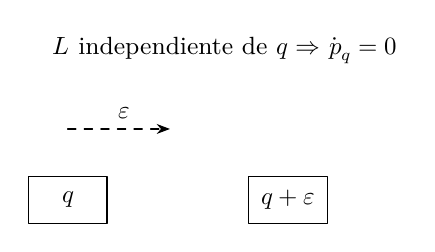
\begin{tikzpicture}[>=Stealth,font=\small,line cap=round,line join=round]
\draw[->,thin,dashed] (-2,0) -- (-0.7,0) node[pos=0.55,above] {$\varepsilon$};
\draw[fill=white] (-2.5,-1.2) rectangle (-1.5,-0.6000000000000001);
\node at (-2,-0.9) {$q$};
\draw[fill=white] (0.30000000000000004,-1.2) rectangle (1.3,-0.6000000000000001);
\node at (0.8,-0.9) {$q+\varepsilon$};
\node at (0,1) {$L$ independiente de $q$ $\Rightarrow$ $\dot p_q=0$};

\end{tikzpicture}
\end{document}
